% Chapter 1: Introduction to Time Series Analysis
% Comprehensive Beamer Presentation with Python-Generated Charts
% Target: Master Students in Statistics and Data Science

\documentclass[9pt, aspectratio=169, t]{beamer}

% Ensure content fits on slides
\setbeamersize{text margin left=8mm, text margin right=8mm}

%=============================================================================
% THEME AND STYLE CONFIGURATION
%=============================================================================
\usetheme{Madrid}
\usecolortheme{seahorse}

% IDA-Inspired Color Palette
\definecolor{MainBlue}{RGB}{26, 58, 110}      % IDA Navy Blue
\definecolor{AccentBlue}{RGB}{42, 82, 140}    % Lighter navy
\definecolor{IDAred}{RGB}{220, 53, 69}        % IDA Red
\definecolor{DarkGray}{RGB}{51, 51, 51}
\definecolor{MediumGray}{RGB}{128, 128, 128}
\definecolor{LightGray}{RGB}{248, 248, 248}
\definecolor{VeryLightGray}{RGB}{235, 235, 235}
\definecolor{Crimson}{RGB}{220, 53, 69}
\definecolor{Forest}{RGB}{46, 125, 50}
\definecolor{Amber}{RGB}{181, 133, 63}

\setbeamercolor{palette primary}{bg=MainBlue, fg=white}
\setbeamercolor{palette secondary}{bg=MainBlue!85, fg=white}
\setbeamercolor{palette tertiary}{bg=MainBlue!70, fg=white}
\setbeamercolor{structure}{fg=MainBlue}
\setbeamercolor{title}{fg=MainBlue}
\setbeamercolor{frametitle}{fg=MainBlue, bg=white}
\setbeamercolor{block title}{bg=MainBlue, fg=white}
\setbeamercolor{block body}{bg=VeryLightGray, fg=DarkGray}
\setbeamercolor{block title alerted}{bg=Crimson, fg=white}
\setbeamercolor{block body alerted}{bg=Crimson!8, fg=DarkGray}
\setbeamercolor{block title example}{bg=Forest, fg=white}
\setbeamercolor{block body example}{bg=Forest!8, fg=DarkGray}
\setbeamercolor{item}{fg=MainBlue}

\setbeamertemplate{navigation symbols}{}

\setbeamertemplate{footline}{
    \leavevmode%
    \hbox{%
        \begin{beamercolorbox}[wd=.333333\paperwidth,ht=2.5ex,dp=1ex,center]{author in head/foot}%
            \usebeamerfont{author in head/foot}\insertshortauthor
        \end{beamercolorbox}%
        \begin{beamercolorbox}[wd=.333333\paperwidth,ht=2.5ex,dp=1ex,center]{title in head/foot}%
            \usebeamerfont{title in head/foot}\insertshorttitle
        \end{beamercolorbox}%
        \begin{beamercolorbox}[wd=.333333\paperwidth,ht=2.5ex,dp=1ex,right]{date in head/foot}%
            \usebeamerfont{date in head/foot}\insertshortdate{}\hspace*{2em}
            \insertframenumber{} / \inserttotalframenumber\hspace*{2ex}
        \end{beamercolorbox}}%
    \vskip0pt%
}

%=============================================================================
% PACKAGES
%=============================================================================
\usepackage{amsmath, amssymb, amsthm}
\usepackage{mathtools}
\usepackage{bm}
\usepackage{tikz}
\usetikzlibrary{arrows.meta, positioning, shapes, calc}
\usepackage{booktabs}
\usepackage{multirow}
\usepackage{array}
\usepackage{graphicx}
\graphicspath{{logos/}{charts/}}

%=============================================================================
% THEOREM ENVIRONMENTS
%=============================================================================
\theoremstyle{definition}
\setbeamertemplate{theorems}[numbered]
\newtheorem{defn}{Definition}
\newtheorem{thm}{Theorem}
\newtheorem{prop}{Proposition}
\newtheorem{rmk}{Remark}

%=============================================================================
% CUSTOM COMMANDS
%=============================================================================
\newcommand{\E}{\mathbb{E}}
\newcommand{\Var}{\text{Var}}
\newcommand{\Cov}{\text{Cov}}
\newcommand{\Corr}{\text{Corr}}
\newcommand{\R}{\mathbb{R}}
\newcommand{\N}{\mathbb{N}}
\newcommand{\Z}{\mathbb{Z}}

%=============================================================================
% TITLE INFORMATION
%=============================================================================
\title[Chapter 1: Introduction to Time Series]{Chapter 1: Introduction to Time Series Analysis}
\subtitle{Bachelor program Faculty of Cybernetics, Statistics and Economic Informatics, Bucharest University of Economic Studies, Romania}
\author[Prof. dr. Daniel Traian Pele]{Prof. dr. Daniel Traian Pele\\[0.2cm]\footnotesize\texttt{danpele@ase.ro}}
\institute{Bucharest University of Economic Studies}
\date{Academic Year 2025--2026}

\begin{document}

%=============================================================================
% TITLE SLIDE
%=============================================================================
\begin{frame}[plain]
    \begin{tikzpicture}[remember picture, overlay]
        \node[anchor=north west] at ([xshift=0.5cm, yshift=-0.3cm]current page.north west) {
            \includegraphics[height=1.1cm]{ase_logo.png}
        };
        \node[anchor=north] at ([yshift=-0.3cm]current page.north) {
            \includegraphics[height=1.1cm]{ai4efin_logo.png}
        };
        \node[anchor=north east] at ([xshift=-0.5cm, yshift=-0.3cm]current page.north east) {
            \includegraphics[height=1.1cm]{msca_logo.png}
        };
    \end{tikzpicture}
    \vspace{0.8cm}

    \begin{center}
        {\Large\textbf{\textcolor{MainBlue}{Time Series Analysis and Forecasting}}}\\[0.3cm]
        {\LARGE\textbf{\textcolor{MainBlue}{Chapter 1: Introduction to Time Series Analysis}}}\\[0.5cm]
        {\small Bachelor program, Faculty of Cybernetics, Statistics and Economic Informatics}\\
        {\small Bucharest University of Economic Studies, Romania}\\[0.5cm]
        {\normalsize Prof.\ dr.\ Daniel Traian Pele}\\
        {\small\texttt{danpele@ase.ro}}\\[0.3cm]
        {\small Academic Year 2025--2026}
    \end{center}

    \begin{tikzpicture}[remember picture, overlay]
        \node[anchor=south west] at ([xshift=1cm, yshift=0.8cm]current page.south west) {
            \includegraphics[height=0.9cm]{ida_logo.png}
        };
        \node[anchor=south] at ([yshift=0.8cm]current page.south) {
            \includegraphics[height=0.9cm]{brc_logo.png}
        };
        \node[anchor=south east] at ([xshift=-1cm, yshift=0.8cm]current page.south east) {
            \includegraphics[height=0.9cm]{acad_logo.png}
        };
    \end{tikzpicture}
\end{frame}

%=============================================================================
% COURSE OBJECTIVES
%=============================================================================
\begin{frame}{Learning Objectives}
    \textbf{\large By the end of this chapter, you will be able to:}
    \vspace{0.15cm}
    \begin{enumerate}
        \item[\textcolor{MainBlue}{\textbf{1.}}] \textbf{Define} time series and distinguish from cross-sectional and panel data
        \vspace{0.08cm}
        \item[\textcolor{MainBlue}{\textbf{2.}}] \textbf{Decompose} time series into trend, seasonal, and residual components
        \vspace{0.08cm}
        \item[\textcolor{MainBlue}{\textbf{3.}}] \textbf{Apply} exponential smoothing (SES, Holt, Holt-Winters, ETS)
        \vspace{0.08cm}
        \item[\textcolor{MainBlue}{\textbf{4.}}] \textbf{Evaluate} forecasts using MAE, RMSE, MAPE; train/validation/test splits
        \vspace{0.08cm}
        \item[\textcolor{MainBlue}{\textbf{5.}}] \textbf{Model} seasonality using dummy variables or Fourier terms
        \vspace{0.08cm}
        \item[\textcolor{MainBlue}{\textbf{6.}}] \textbf{Handle} trend and seasonality through detrending and adjustment
        \vspace{0.08cm}
        \item[\textcolor{MainBlue}{\textbf{7.}}] \textbf{Understand} stochastic processes and stationarity
        \vspace{0.08cm}
        \item[\textcolor{MainBlue}{\textbf{8.}}] \textbf{Compute} ACF/PACF and conduct stationarity tests (ADF, KPSS)
    \end{enumerate}
\end{frame}

%=============================================================================
% TABLE OF CONTENTS
%=============================================================================
\begin{frame}{Chapter Outline}
    \tableofcontents
\end{frame}

%=============================================================================
% SECTION 1: WHAT IS A TIME SERIES
%=============================================================================
\section{What is a Time Series?}

\begin{frame}{Definition of a Time Series}
    \begin{defn}[Time Series]
        A \textbf{time series} is a sequence of observations $\{X_t\}$ indexed by time:
        \[
            \{X_t : t \in \mathcal{T}\}
        \]
        where $\mathcal{T}$ is an index set representing time points.
    \end{defn}

    \vspace{0.3cm}

    \textbf{Key characteristics:}
    \begin{itemize}
        \item \textbf{Ordered}: Observations have a natural temporal ordering
        \item \textbf{Dependent}: Consecutive observations are typically correlated
        \item \textbf{Discrete} or \textbf{Continuous}: Time index can be discrete ($t = 1, 2, 3, \ldots$) or continuous
    \end{itemize}

    \vspace{0.3cm}

    \textbf{Notation:}
    \begin{itemize}
        \item $X_t$ = observation at time $t$
        \item $\{X_t\}_{t=1}^{T}$ = finite time series with $T$ observations
    \end{itemize}
\end{frame}

\begin{frame}{Time Series: Visual Definition}
    \begin{center}
        \includegraphics[width=0.78\textwidth]{timeseries_definition.pdf}
    \end{center}
    \vspace{-0.2cm}
    \small Each point $X_t$ represents a measurement at discrete time $t$. Data: S\&P 500 (2024).
\end{frame}

\begin{frame}{Types of Data: Comparison}
    \begin{center}
        \includegraphics[width=0.78\textwidth]{data_types_comparison.pdf}
    \end{center}

    \vspace{0.2cm}
    \begin{center}
    \small
    \begin{tabular}{lccc}
        \toprule
        \textbf{Data Type} & \textbf{Units ($N$)} & \textbf{Time ($T$)} & \textbf{Example} \\
        \midrule
        Cross-sectional & Many & 1 & Survey of 1000 households \\
        Time series & 1 & Many & Daily S\&P 500 prices \\
        Panel & Many & Many & GDP of 50 countries, 20 years \\
        \bottomrule
    \end{tabular}
    \end{center}
\end{frame}

\begin{frame}{Examples of Time Series Data}
    \begin{center}
        \includegraphics[width=0.78\textwidth]{multiple_assets.pdf}
    \end{center}
    \vspace{-0.2cm}
    \centering\small Real financial data from Yahoo Finance (2019--2025). Normalized to base 100.
\end{frame}

%=============================================================================
% SECTION 2: TIME SERIES DECOMPOSITION
%=============================================================================
\section{Time Series Decomposition}

\begin{frame}{Why Decompose a Time Series?}
    \textbf{Decomposition} separates a time series into interpretable components:

    \vspace{0.3cm}

    \begin{columns}[T]
        \begin{column}{0.48\textwidth}
            \textbf{Goals:}
            \begin{itemize}
                \item Understand underlying patterns
                \item Remove seasonality for modeling
                \item Identify trend direction
                \item Isolate irregular fluctuations
                \item Improve forecasting accuracy
            \end{itemize}
        \end{column}
        \begin{column}{0.48\textwidth}
            \textbf{Components:}
            \begin{itemize}
                \item $T_t$ = \textbf{Trend}: Long-term movement
                \item $S_t$ = \textbf{Seasonal}: Regular periodic pattern
                \item $C_t$ = \textbf{Cyclical}: Business cycle fluctuations
                \item $\varepsilon_t$ = \textbf{Residual}: Random noise
            \end{itemize}
        \end{column}
    \end{columns}

    \vspace{0.4cm}

    \begin{block}{Classical Decomposition Models}
        \begin{itemize}
            \item \textbf{Additive}: $X_t = T_t + S_t + \varepsilon_t$
            \item \textbf{Multiplicative}: $X_t = T_t \times S_t \times \varepsilon_t$
        \end{itemize}
    \end{block}
\end{frame}

\begin{frame}{The Cyclical Component}
    \textbf{Cyclical component} $C_t$: Medium-term fluctuations (2--10 years)

    \vspace{0.3cm}

    \begin{columns}[T]
        \begin{column}{0.48\textwidth}
            \textbf{Characteristics:}
            \begin{itemize}
                \item Business cycle fluctuations
                \item No fixed period (unlike seasonal)
                \item Duration varies: 2--10 years
                \item Amplitude varies over time
            \end{itemize}
        \end{column}
        \begin{column}{0.48\textwidth}
            \textbf{Examples:}
            \begin{itemize}
                \item Economic expansions/recessions
                \item Credit cycles
                \item Real estate cycles
                \item Commodity price cycles
            \end{itemize}
        \end{column}
    \end{columns}

    \vspace{0.3cm}

    \begin{alertblock}{Practical Note}
        Often combined with trend as \textbf{trend-cycle} component because:
        \begin{itemize}
            \item Difficult to separate from trend with short data
            \item Many decomposition methods estimate $T_t + C_t$ together
        \end{itemize}
    \end{alertblock}
\end{frame}

\begin{frame}{Additive Decomposition Model}
    \textbf{Formula:} \quad $X_t = T_t + S_t + \varepsilon_t$

    \vspace{0.3cm}

    \textbf{When to use:}
    \begin{itemize}
        \item Seasonal fluctuations are \textbf{constant} over time
        \item Variance of the series is \textbf{stable}
    \end{itemize}

    \vspace{0.3cm}

    \textbf{Properties:}
    \begin{itemize}
        \item $\E[\varepsilon_t] = 0$ (zero mean residuals)
        \item $\sum_{j=1}^{s} S_j = 0$ (seasonal sums to zero)
        \item Units of $S_t$ same as $X_t$
    \end{itemize}
\end{frame}

\begin{frame}{Additive Decomposition: Visualization}
    \begin{center}
        \includegraphics[width=0.78\textwidth]{ts_components_synthetic.pdf}
    \end{center}
\end{frame}

\begin{frame}{Multiplicative Decomposition Model}
    \textbf{Formula:} \quad $X_t = T_t \times S_t \times \varepsilon_t$

    \vspace{0.3cm}

    \textbf{When to use:}
    \begin{itemize}
        \item Seasonal fluctuations \textbf{grow} with series level
        \item Variance \textbf{increases} over time
    \end{itemize}

    \vspace{0.3cm}

    \textbf{Properties:}
    \begin{itemize}
        \item $\E[\varepsilon_t] = 1$ (residuals centered at 1)
        \item $\frac{1}{s}\sum S_j = 1$ (seasonal averages to 1)
        \item $S_t$ is a ratio (dimensionless)
    \end{itemize}

    \vspace{0.3cm}

    \textbf{Tip:} Log transform converts to additive model.
\end{frame}

\begin{frame}{Multiplicative Decomposition: Real Data}
    \begin{center}
        \includegraphics[width=0.72\textwidth]{airline_decomposition.pdf}
    \end{center}
    \vspace{-0.3cm}
    \centering\small Classic Box-Jenkins airline passengers dataset (1949--1960).
\end{frame}

\begin{frame}{Additive vs Multiplicative: Comparison}
    \begin{center}
        \includegraphics[width=0.78\textwidth]{additive_vs_multiplicative.pdf}
    \end{center}

    \vspace{0.2cm}
    \small\textbf{Key difference:} In multiplicative model, seasonal component is a \textit{ratio} (centered at 1), while in additive model it's in \textit{absolute units} (centered at 0).
\end{frame}

\begin{frame}{Trend Estimation: Moving Average}
    \begin{defn}[Centered Moving Average]
        The \textbf{centered moving average} of order $2q+1$ is:
        \[
            \hat{T}_t = \frac{1}{2q+1} \sum_{j=-q}^{q} X_{t+j}
        \]
    \end{defn}

    \vspace{0.2cm}

    \textbf{For seasonal data:}
    \begin{itemize}
        \item If period $s$ is \textbf{odd}: simple average over $s$ observations
        \item If period $s$ is \textbf{even} (e.g., 12): use $2 \times s$ MA with half-weights at ends
    \end{itemize}

    \vspace{0.2cm}

    \textbf{Properties:}
    \begin{itemize}
        \item Smooths out seasonal and random fluctuations
        \item Larger window $\Rightarrow$ smoother trend
        \item Trade-off: lose data at endpoints
    \end{itemize}
\end{frame}

\begin{frame}{Moving Average: Effect of Window Size}
    \begin{center}
        \includegraphics[width=0.78\textwidth]{moving_average_trend.pdf}
    \end{center}
    \vspace{-0.2cm}
    \small Larger window sizes produce smoother trends but lose more data at boundaries.
\end{frame}

\begin{frame}{Classical Decomposition Algorithm}
    \textbf{Steps for Multiplicative Decomposition:}

    \vspace{0.2cm}

    \begin{enumerate}
        \item \textbf{Estimate Trend}: $\hat{T}_t = MA_s(X_t)$

        \vspace{0.15cm}

        \item \textbf{Detrend}: $D_t = X_t / \hat{T}_t$

        \vspace{0.15cm}

        \item \textbf{Estimate Seasonal}: Average $D_t$ for each season $j$
        \[
            \hat{S}_j = \text{mean}(D_t \text{ for all } t \text{ in season } j)
        \]

        \vspace{0.15cm}

        \item \textbf{Normalize}: Scale so $\frac{1}{s}\sum_{j=1}^{s} \hat{S}_j = 1$

        \vspace{0.15cm}

        \item \textbf{Compute Residuals}: $\hat{\varepsilon}_t = X_t / (\hat{T}_t \times \hat{S}_t)$
    \end{enumerate}
\end{frame}

\begin{frame}{Seasonal Indices: Interpretation}
    \begin{center}
        \includegraphics[width=0.78\textwidth]{seasonal_pattern.pdf}
    \end{center}

    \vspace{0.2cm}
    \small\textbf{Interpretation:} $S_t > 1$ means above-average activity; $S_t < 1$ means below-average. Airline data shows peak travel in July--August.
\end{frame}

\begin{frame}{STL Decomposition: A Modern Approach}
    \begin{defn}[STL - Seasonal-Trend decomposition using LOESS]
        \textbf{STL} uses locally weighted regression (LOESS) to estimate components:
        \[
            X_t = T_t + S_t + R_t
        \]
    \end{defn}

    \vspace{0.2cm}

    \textbf{Advantages over classical decomposition:}
    \begin{itemize}
        \item Handles \textbf{any seasonal period} (not just 4 or 12)
        \item Seasonal component can \textbf{change over time}
        \item \textbf{Robust} to outliers (with robust=True option)
        \item Provides \textbf{smooth} trend estimates
    \end{itemize}

    \vspace{0.2cm}

    \textbf{Key parameters:}
    \begin{itemize}
        \item \texttt{period}: Seasonal period (e.g., 12 for monthly)
        \item \texttt{seasonal}: Window for seasonal smoothing (odd integer)
        \item \texttt{robust}: Use robust fitting to downweight outliers
    \end{itemize}
\end{frame}

\begin{frame}{STL Decomposition: Example}
    \begin{center}
        \includegraphics[width=0.78\textwidth]{stl_decomposition.pdf}
    \end{center}
\end{frame}

%=============================================================================
% SECTION 3: EXPONENTIAL SMOOTHING METHODS
%=============================================================================
\section{Exponential Smoothing Methods}

\begin{frame}{Exponential Smoothing: Overview}
    \textbf{Exponential smoothing} methods produce forecasts based on weighted averages of past observations, with weights decaying exponentially.

    \vspace{0.3cm}

    \begin{block}{Why Exponential Smoothing?}
        \begin{itemize}
            \item Simple yet effective forecasting methods
            \item More recent observations get higher weights
            \item Handles trend and seasonality
            \item Foundation for ETS models
        \end{itemize}
    \end{block}

    \vspace{0.3cm}

    \textbf{Three main methods:}
    \begin{enumerate}
        \item \textbf{Simple Exponential Smoothing (SES)}: Level only
        \item \textbf{Holt's Method}: Level + Trend
        \item \textbf{Holt-Winters}: Level + Trend + Seasonality
    \end{enumerate}
\end{frame}

\begin{frame}{Simple Exponential Smoothing (SES)}
    \textbf{Forecast:} \quad $\hat{X}_{t+1|t} = \alpha X_t + (1-\alpha)\hat{X}_{t|t-1}$

    \vspace{0.3cm}

    where $\alpha \in (0,1)$ is the \textbf{smoothing parameter}.

    \vspace{0.3cm}

    \textbf{How it works:}
    \begin{itemize}
        \item Weights decay exponentially into the past
        \item Large $\alpha$: responsive to recent changes
        \item Small $\alpha$: smoother, more stable forecasts
    \end{itemize}

    \vspace{0.3cm}

    \textbf{Level form:} \quad $\ell_t = \alpha X_t + (1-\alpha)\ell_{t-1}$
\end{frame}

\begin{frame}{Simple Exponential Smoothing: Effect of $\alpha$}
    \begin{center}
        \includegraphics[width=0.78\textwidth]{simple_exp_smoothing.pdf}
    \end{center}
    \vspace{-0.2cm}
    \small Smaller $\alpha$ produces smoother forecasts; larger $\alpha$ follows data more closely.
\end{frame}

\begin{frame}{Holt's Linear Trend Method}
    Extends SES to capture \textbf{linear trend} using two equations:

    \vspace{0.3cm}

    \textbf{Level:} \quad $\ell_t = \alpha X_t + (1-\alpha)(\ell_{t-1} + b_{t-1})$

    \vspace{0.2cm}

    \textbf{Trend:} \quad $b_t = \beta^*(\ell_t - \ell_{t-1}) + (1-\beta^*)b_{t-1}$

    \vspace{0.3cm}

    \textbf{Forecast:} \quad $\hat{X}_{t+h|t} = \ell_t + h \cdot b_t$

    \vspace{0.3cm}

    \textbf{Parameters:}
    \begin{itemize}
        \item $\alpha \in (0,1)$: Level smoothing parameter
        \item $\beta^* \in (0,1)$: Trend smoothing parameter
        \item $\ell_t$: Estimated level at time $t$
        \item $b_t$: Estimated trend (slope) at time $t$
    \end{itemize}
\end{frame}

\begin{frame}{Holt's Method: Visualization}
    \begin{center}
        \includegraphics[width=0.78\textwidth]{holt_method.pdf}
    \end{center}
    \vspace{-0.2cm}
    \small Holt's method captures both level and trend, projecting them into the forecast horizon.
\end{frame}

\begin{frame}{Holt-Winters Seasonal Method}
    Extends Holt's method to include \textbf{seasonality} with three equations:

    \vspace{0.2cm}

    \textbf{Level:} \quad $\ell_t = \alpha(X_t - S_{t-s}) + (1-\alpha)(\ell_{t-1} + b_{t-1})$

    \vspace{0.1cm}

    \textbf{Trend:} \quad $b_t = \beta^*(\ell_t - \ell_{t-1}) + (1-\beta^*)b_{t-1}$

    \vspace{0.1cm}

    \textbf{Seasonal:} \quad $S_t = \gamma(X_t - \ell_t) + (1-\gamma)S_{t-s}$

    \vspace{0.3cm}

    \textbf{Forecast:} \quad $\hat{X}_{t+h|t} = \ell_t + h \cdot b_t + S_{t+h-s(k+1)}$

    \vspace{0.3cm}

    \textbf{Parameters:}
    \begin{itemize}
        \item $\alpha$: Level smoothing
        \item $\beta^*$: Trend smoothing
        \item $\gamma$: Seasonal smoothing
        \item $s$: Seasonal period (e.g., 12 for monthly)
    \end{itemize}
\end{frame}

\begin{frame}{Holt-Winters: Capturing Seasonality}
    \begin{center}
        \includegraphics[width=0.78\textwidth]{holt_winters.pdf}
    \end{center}
    \vspace{-0.2cm}
    \small Holt-Winters decomposes the series and produces seasonal forecasts.
\end{frame}

\begin{frame}{ETS Framework: Error-Trend-Seasonal}
    \begin{defn}[ETS Models]
        The \textbf{ETS framework} generalizes exponential smoothing with explicit error structure:
        \[
            \text{ETS}(E, T, S)
        \]
        where each component can be:
    \end{defn}

    \vspace{0.2cm}

    \begin{center}
    \small
    \begin{tabular}{llll}
        \toprule
        \textbf{Component} & \textbf{N} & \textbf{A} & \textbf{M} \\
        \midrule
        Error (E) & -- & Additive & Multiplicative \\
        Trend (T) & None & Additive & Multiplicative \\
        Seasonal (S) & None & Additive & Multiplicative \\
        \bottomrule
    \end{tabular}
    \end{center}

    \vspace{0.2cm}

    \textbf{Examples:}
    \begin{itemize}
        \item ETS(A,N,N) = Simple Exponential Smoothing
        \item ETS(A,A,N) = Holt's Linear Method
        \item ETS(A,A,A) = Holt-Winters Additive
        \item ETS(M,A,M) = Multiplicative errors, additive trend, multiplicative seasonal
    \end{itemize}
\end{frame}

\begin{frame}{ETS Model Selection}
    \begin{center}
        \includegraphics[width=0.78\textwidth]{ets_components.pdf}
    \end{center}
    \vspace{-0.2cm}
    \small The ETS framework provides a systematic way to choose the best model using AIC/BIC.
\end{frame}

\begin{frame}{Damped Trend Methods}
    Introduces \textbf{damping parameter} $\phi \in (0,1)$ to prevent over-projection:

    \vspace{0.2cm}

    \textbf{Level:} \quad $\ell_t = \alpha X_t + (1-\alpha)(\ell_{t-1} + \phi b_{t-1})$

    \vspace{0.1cm}

    \textbf{Trend:} \quad $b_t = \beta^*(\ell_t - \ell_{t-1}) + (1-\beta^*)\phi b_{t-1}$

    \vspace{0.2cm}

    \textbf{Forecast:} \quad $\hat{X}_{t+h|t} = \ell_t + \phi\frac{1-\phi^h}{1-\phi}b_t$

    \vspace{0.3cm}

    \textbf{Key insight:}
    \begin{itemize}
        \item As $h \to \infty$: forecast $\to \ell_t + \frac{\phi}{1-\phi}b_t$ (constant)
        \item Prevents unrealistic long-term extrapolation
        \item Often best for longer forecast horizons
    \end{itemize}
\end{frame}

%=============================================================================
% SECTION 4: FORECAST EVALUATION
%=============================================================================
\section{Forecast Evaluation}

\begin{frame}{Forecast Accuracy Metrics}
    \textbf{Forecast Error:} $e_t = X_t - \hat{X}_t$ (actual minus predicted)

    \vspace{0.3cm}

    \begin{columns}[T]
        \begin{column}{0.48\textwidth}
            \textbf{Scale-Dependent:}
            \begin{itemize}
                \item MAE $= \frac{1}{n}\sum|e_t|$
                \item MSE $= \frac{1}{n}\sum e_t^2$
                \item RMSE $= \sqrt{\text{MSE}}$
            \end{itemize}
        \end{column}
        \begin{column}{0.48\textwidth}
            \textbf{Scale-Independent:}
            \begin{itemize}
                \item MAPE $= \frac{100}{n}\sum\left|\frac{e_t}{X_t}\right|$
                \item sMAPE (symmetric)
            \end{itemize}
        \end{column}
    \end{columns}

    \vspace{0.3cm}

    \begin{alertblock}{Which to use?}
        \begin{itemize}
            \item Same series: RMSE, MAE
            \item Compare across series: MAPE, sMAPE
        \end{itemize}
    \end{alertblock}
\end{frame}

\begin{frame}{Comparing Forecast Methods}
    \begin{center}
        \includegraphics[width=0.78\textwidth]{forecast_accuracy_metrics.pdf}
    \end{center}
    \vspace{-0.2cm}
    \small\textbf{Left:} Comparing SES, Holt, and Holt-Winters forecasts. \textbf{Right:} Error metrics for each method.
\end{frame}

\begin{frame}{Residual Diagnostics}
    \textbf{Good forecasts} should have residuals that are:

    \vspace{0.2cm}

    \begin{enumerate}
        \item \textbf{Zero mean}: $\E[e_t] = 0$ (unbiased)
        \item \textbf{Uncorrelated}: $\Cov(e_t, e_{t-k}) = 0$ for $k \neq 0$
        \item \textbf{Constant variance}: $\Var(e_t) = \sigma^2$ (homoscedastic)
        \item \textbf{Normally distributed}: $e_t \sim N(0, \sigma^2)$ (for prediction intervals)
    \end{enumerate}

    \vspace{0.3cm}

    \textbf{Diagnostic tests:}
    \begin{itemize}
        \item \textbf{Ljung-Box test}: Tests for autocorrelation in residuals
        \[
            Q = T(T+2)\sum_{k=1}^{h}\frac{\hat{\rho}_k^2}{T-k} \sim \chi^2_h
        \]
        \item \textbf{Jarque-Bera test}: Tests for normality
    \end{itemize}
\end{frame}

\begin{frame}{Residual Diagnostics: Visualization}
    \begin{center}
        \includegraphics[width=0.78\textwidth]{residual_diagnostics.pdf}
    \end{center}
\end{frame}

\begin{frame}{Time Series Cross-Validation}
    \textbf{Standard CV} doesn't work for time series (temporal dependence).

    \vspace{0.2cm}

    \textbf{Rolling Origin CV:} Expanding windows
    \begin{enumerate}
        \item Train on $\{X_1, \ldots, X_t\}$, forecast $\hat{X}_{t+h}$
        \item Increment $t$, repeat
    \end{enumerate}

    \begin{center}
        \includegraphics[width=0.72\textwidth]{cross_validation_forecast.pdf}
    \end{center}
\end{frame}

\begin{frame}{Train / Validation / Test Split}
    \textbf{Three-way split} for model development:

    \vspace{0.2cm}

    \begin{columns}[T]
        \begin{column}{0.32\textwidth}
            \textbf{\textcolor{MainBlue}{Training Set}}
            \begin{itemize}
                \item Fit model parameters
                \item Largest portion (60--80\%)
                \item Used for estimation
            \end{itemize}
        \end{column}
        \begin{column}{0.32\textwidth}
            \textbf{\textcolor{Forest}{Validation Set}}
            \begin{itemize}
                \item Tune hyperparameters
                \item Compare models
                \item Select best approach
            \end{itemize}
        \end{column}
        \begin{column}{0.32\textwidth}
            \textbf{\textcolor{Crimson}{Test Set}}
            \begin{itemize}
                \item Final evaluation only
                \item Never used for tuning
                \item Unbiased performance
            \end{itemize}
        \end{column}
    \end{columns}

    \vspace{0.3cm}

    \begin{center}
        \includegraphics[width=0.78\textwidth]{train_test_validation.pdf}
    \end{center}
\end{frame}

\begin{frame}{Model Development Workflow}
    \begin{center}
    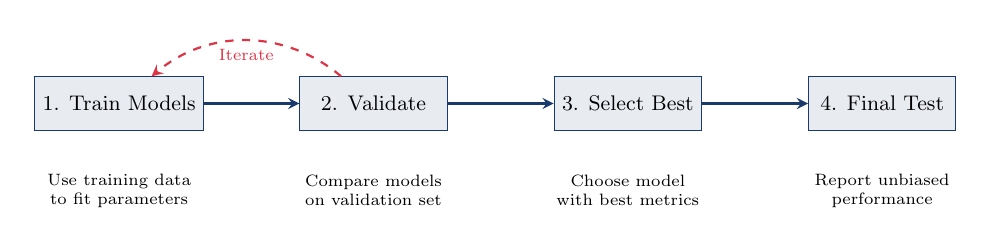
\begin{tikzpicture}[node distance=1.8cm, scale=0.85, transform shape]
        \tikzstyle{process} = [rectangle, minimum width=2.2cm, minimum height=0.8cm, text centered, draw=MainBlue, fill=MainBlue!10, font=\small]
        \tikzstyle{arrow} = [->, >=stealth, thick, MainBlue]

        % Nodes
        \node (train) [process] {1. Train Models};
        \node (validate) [process, right of=train, xshift=2cm] {2. Validate};
        \node (select) [process, right of=validate, xshift=2cm] {3. Select Best};
        \node (test) [process, right of=select, xshift=2cm] {4. Final Test};

        % Arrows
        \draw [arrow] (train) -- (validate);
        \draw [arrow] (validate) -- (select);
        \draw [arrow] (select) -- (test);

        % Feedback loop
        \draw [arrow, dashed, Crimson] (validate) to[bend right=40] node[below, font=\scriptsize] {Iterate} (train);

        % Labels below
        \node [below of=train, yshift=0.5cm, font=\scriptsize, text width=2.5cm, align=center] {Use training data\\to fit parameters};
        \node [below of=validate, yshift=0.5cm, font=\scriptsize, text width=2.5cm, align=center] {Compare models\\on validation set};
        \node [below of=select, yshift=0.5cm, font=\scriptsize, text width=2.5cm, align=center] {Choose model\\with best metrics};
        \node [below of=test, yshift=0.5cm, font=\scriptsize, text width=2.5cm, align=center] {Report unbiased\\performance};
    \end{tikzpicture}
    \end{center}

    \vspace{0.3cm}

    \begin{alertblock}{Critical Rule}
        \textbf{Never} use test set for model selection! This causes \textit{data leakage} and overly optimistic performance estimates.
    \end{alertblock}
\end{frame}

\begin{frame}{Real Data: Forecast Comparison}
    \begin{center}
        \includegraphics[width=0.78\textwidth]{real_data_forecast_comparison.pdf}
    \end{center}
    \vspace{-0.2cm}
    \small Airline passengers data: Holt-Winters Multiplicative performs best for seasonal data.
\end{frame}

\begin{frame}{Forecast Performance Across Datasets}
    \begin{center}
        \includegraphics[width=0.78\textwidth]{multiple_series_comparison.pdf}
    \end{center}
    \vspace{-0.2cm}
    \small Different series require different models. Seasonal data needs seasonal methods.
\end{frame}

%=============================================================================
% SECTION 5: MODELING SEASONALITY
%=============================================================================
\section{Modeling Seasonality}

\begin{frame}{Modeling Seasonality: Two Approaches}
    \begin{columns}[T]
        \begin{column}{0.48\textwidth}
            \textbf{1. Dummy Variables:}

            \vspace{0.1cm}
            $X_t = \mu + \sum_{j=1}^{s-1}\gamma_j D_{jt} + \varepsilon_t$

            \vspace{0.2cm}
            \begin{itemize}
                \item $D_{jt} = 1$ if $t$ in season $j$
                \item $s-1$ parameters
                \item Any seasonal pattern
            \end{itemize}
        \end{column}
        \begin{column}{0.48\textwidth}
            \textbf{2. Fourier Terms:}

            \vspace{0.1cm}
            $X_t = \mu + \sum_{k=1}^{K}[\alpha_k\sin(\cdot) + \beta_k\cos(\cdot)]$

            \vspace{0.2cm}
            \begin{itemize}
                \item Sinusoidal functions
                \item $2K$ parameters
                \item Smooth patterns
            \end{itemize}
        \end{column}
    \end{columns}

    \vspace{0.3cm}

    \begin{alertblock}{Trade-off}
        Dummies: any pattern, more parameters. Fourier: smooth, fewer parameters.
    \end{alertblock}
\end{frame}

\begin{frame}{Dummy Variables vs Fourier Terms}
    \begin{center}
        \includegraphics[width=0.78\textwidth]{seasonality_fourier_dummies.pdf}
    \end{center}
\end{frame}

\begin{frame}{Choosing Between Dummies and Fourier}
    \begin{center}
    \small
    \begin{tabular}{lcc}
        \toprule
        \textbf{Criterion} & \textbf{Dummies} & \textbf{Fourier} \\
        \midrule
        Parameters (monthly) & 11 & $2K$ (often 4--6) \\
        Seasonal pattern & Any shape & Smooth/sinusoidal \\
        Interpretation & Direct (month effects) & Frequency components \\
        High-frequency seasons & Many parameters & Efficient \\
        Multiple seasonality & Complex & Easy (add terms) \\
        \bottomrule
    \end{tabular}
    \end{center}

    \vspace{0.3cm}

    \textbf{Guidelines:}
    \begin{itemize}
        \item Use \textbf{dummies} when seasonal pattern is irregular or you need interpretable coefficients
        \item Use \textbf{Fourier} for smooth patterns, high-frequency seasonality (daily, hourly), or multiple seasonal periods
        \item \textbf{Fourier terms} are used in TBATS models and Facebook Prophet
    \end{itemize}
\end{frame}

%=============================================================================
% SECTION 6: HANDLING TREND AND SEASONALITY
%=============================================================================
\section{Handling Trend and Seasonality}

\begin{frame}{Why Remove Trend and Seasonality?}
    \textbf{Before modeling}, we often need to make series stationary:

    \vspace{0.3cm}

    \begin{columns}[T]
        \begin{column}{0.48\textwidth}
            \textbf{Reasons to detrend:}
            \begin{itemize}
                \item Stationarity requirement
                \item Focus on fluctuations
                \item Avoid spurious regression
                \item Enable valid inference
            \end{itemize}
        \end{column}
        \begin{column}{0.48\textwidth}
            \textbf{Reasons to deseasonalize:}
            \begin{itemize}
                \item Reveal underlying trend
                \item Compare across seasons
                \item Simplify modeling
                \item Focus on irregular component
            \end{itemize}
        \end{column}
    \end{columns}

    \vspace{0.4cm}

    \begin{alertblock}{Important}
        After modeling the detrended/deseasonalized series, we must \textbf{reverse the transformation} for forecasting.
    \end{alertblock}
\end{frame}

\begin{frame}{Trend Removal Methods}
    \textbf{Six common detrending approaches:}

    \vspace{0.2cm}

    \begin{enumerate}
        \item \textbf{Differencing}: $\Delta X_t = X_t - X_{t-1}$
        \item \textbf{Linear regression}: Fit $\hat{T}_t = \hat{\beta}_0 + \hat{\beta}_1 t$
        \item \textbf{Polynomial}: Fit higher-order polynomial
        \item \textbf{HP Filter}: Balance fit vs smoothness
        \item \textbf{Moving average}: $\hat{T}_t = MA_q(X_t)$
        \item \textbf{LOESS}: Local polynomial regression
    \end{enumerate}

    \vspace{0.3cm}

    \textbf{Choice depends on:}
    \begin{itemize}
        \item Nature of trend (deterministic vs stochastic)
        \item Purpose (forecasting vs analysis)
    \end{itemize}
\end{frame}

\begin{frame}{Detrending Methods: Comparison}
    \begin{center}
        \includegraphics[width=0.78\textwidth]{detrending_methods.pdf}
    \end{center}
\end{frame}

\begin{frame}{Trend Estimation: Multiple Approaches}
    \begin{center}
        \includegraphics[width=0.78\textwidth]{trend_estimation_comparison.pdf}
    \end{center}
    \vspace{-0.2cm}
    \small Different methods capture trend at varying levels of smoothness.
\end{frame}

\begin{frame}{Seasonality Removal Methods}
    \textbf{Four approaches to remove seasonality:}

    \vspace{0.3cm}

    \begin{enumerate}
        \item \textbf{Seasonal differencing}: $\Delta_s X_t = X_t - X_{t-s}$

        \vspace{0.2cm}

        \item \textbf{Division} (multiplicative): $X_t^{adj} = X_t / \hat{S}_t$

        \vspace{0.2cm}

        \item \textbf{Subtraction} (additive): $X_t^{adj} = X_t - \hat{S}_t$

        \vspace{0.2cm}

        \item \textbf{X-13ARIMA-SEATS}: Government statistical method
    \end{enumerate}

    \vspace{0.3cm}

    \textbf{Seasonal period} $s$: Monthly $\Rightarrow s=12$; Quarterly $\Rightarrow s=4$
\end{frame}

\begin{frame}{Seasonal Adjustment: Visualization}
    \begin{center}
        \includegraphics[width=0.78\textwidth]{seasonal_adjustment.pdf}
    \end{center}
\end{frame}

\begin{frame}{Deterministic vs Stochastic Trend}
    \begin{columns}[T]
        \begin{column}{0.48\textwidth}
            \textbf{Deterministic Trend:}
            \[
                X_t = \beta_0 + \beta_1 t + \varepsilon_t
            \]
            \begin{itemize}
                \item Trend is a function of time
                \item Detrend by regression
                \item $\varepsilon_t$ is stationary
            \end{itemize}
        \end{column}
        \begin{column}{0.48\textwidth}
            \textbf{Stochastic Trend:}
            \[
                X_t = X_{t-1} + \varepsilon_t
            \]
            \begin{itemize}
                \item Random walk component
                \item Detrend by differencing
                \item $\Delta X_t$ is stationary
            \end{itemize}
        \end{column}
    \end{columns}

    \vspace{0.3cm}

    \begin{alertblock}{Wrong Method = Problems}
        \begin{itemize}
            \item Differencing deterministic trend $\Rightarrow$ over-differencing
            \item Regression on stochastic trend $\Rightarrow$ spurious regression
        \end{itemize}
    \end{alertblock}
\end{frame}

\begin{frame}{Example: Deterministic Trend}
    \begin{center}
        \includegraphics[width=0.78\textwidth]{deterministic_trend_example.pdf}
    \end{center}
    \vspace{-0.1cm}
    \small \textbf{Key:} Use \textcolor{Crimson}{regression} to remove trend $\rightarrow$ residuals are stationary (ACF decays quickly).
\end{frame}

\begin{frame}{Example: Stochastic Trend (Random Walk)}
    \begin{center}
        \includegraphics[width=0.78\textwidth]{stochastic_trend_example.pdf}
    \end{center}
    \vspace{-0.1cm}
    \small \textbf{Key:} Use \textcolor{Crimson}{differencing} to remove trend $\rightarrow$ differences are stationary (white noise).
\end{frame}

\begin{frame}{Side-by-Side Comparison}
    \begin{center}
        \includegraphics[width=0.72\textwidth]{trend_comparison_sidebyside.pdf}
    \end{center}
    \vspace{-0.2cm}
    \small \textbf{Remember:} Deterministic $\rightarrow$ regression. Stochastic $\rightarrow$ differencing.
\end{frame}

%=============================================================================
% SECTION 7: STOCHASTIC PROCESSES
%=============================================================================
\section{Stochastic Processes}

\begin{frame}{Stochastic Process: Definition}
    \begin{defn}[Stochastic Process]
        A \textbf{stochastic process} is a collection of random variables indexed by time:
        \[
            \{X_t(\omega) : t \in \mathcal{T}, \omega \in \Omega\}
        \]
        where $\Omega$ is the sample space of possible outcomes.
    \end{defn}

    \vspace{0.3cm}

    \textbf{Two perspectives:}
    \begin{itemize}
        \item \textbf{Fixed $\omega$}: A \textit{realization} or \textit{sample path} $\{X_t(\omega)\}_{t \in \mathcal{T}}$
        \item \textbf{Fixed $t$}: A \textit{random variable} $X_t$ with distribution $F_t(x)$
    \end{itemize}

    \vspace{0.3cm}

    \textbf{Key insight:} A time series we observe is \textbf{one realization} of the underlying stochastic process. We use this single realization to infer properties of the process.
\end{frame}

\begin{frame}{Realizations vs Ensemble}
    \begin{center}
        \includegraphics[width=0.78\textwidth]{realizations_ensemble.pdf}
    \end{center}
    \vspace{-0.2cm}
    \small\textbf{Left:} Multiple realizations from the same process. \textbf{Right:} Distribution at fixed time $t=50$ (ensemble average).
\end{frame}

\begin{frame}{Moments of a Stochastic Process}
    \textbf{First two moments characterize weak properties:}

    \vspace{0.2cm}

    \textbf{Mean Function:} \quad $\mu_t = \E[X_t]$

    \vspace{0.2cm}

    \textbf{Autocovariance Function (ACVF):}
    \[
        \gamma(t, s) = \Cov(X_t, X_s) = \E[(X_t - \mu_t)(X_s - \mu_s)]
    \]

    \vspace{0.2cm}

    \textbf{Autocorrelation Function (ACF):}
    \[
        \rho(t, s) = \frac{\gamma(t, s)}{\sqrt{\Var(X_t) \cdot \Var(X_s)}}
    \]

    \vspace{0.2cm}

    \textbf{Properties:} $\rho(t, s) \in [-1, 1]$ and $\rho(t, t) = 1$
\end{frame}

%=============================================================================
% SECTION 4: STATIONARITY
%=============================================================================
\section{Stationarity}

\begin{frame}{Why Stationarity Matters}
    \textbf{Stationarity} is a fundamental assumption for time series analysis:

    \vspace{0.3cm}

    \begin{columns}[T]
        \begin{column}{0.48\textwidth}
            \textbf{\textcolor{Crimson}{Without Stationarity:}}
            \begin{itemize}
                \item Mean, variance change over time
                \item Past may not predict future
                \item Standard methods fail
                \item Spurious correlations
            \end{itemize}
        \end{column}
        \begin{column}{0.48\textwidth}
            \textbf{\textcolor{Forest}{With Stationarity:}}
            \begin{itemize}
                \item Statistical properties constant
                \item Can estimate from one realization
                \item Valid inference possible
                \item Models are meaningful
            \end{itemize}
        \end{column}
    \end{columns}

    \vspace{0.4cm}

    \begin{alertblock}{Key Principle}
        Most time series models (ARMA, ARIMA, etc.) require stationarity. Non-stationary series must be transformed (e.g., differencing) before modeling.
    \end{alertblock}
\end{frame}

\begin{frame}{Strict Stationarity}
    \begin{defn}[Strict (Strong) Stationarity]
        A process $\{X_t\}$ is \textbf{strictly stationary} if for all $k$, all $t_1, \ldots, t_k$, and all $h$:
        \[
            (X_{t_1}, X_{t_2}, \ldots, X_{t_k}) \stackrel{d}{=} (X_{t_1+h}, X_{t_2+h}, \ldots, X_{t_k+h})
        \]
    \end{defn}

    \vspace{0.3cm}

    \textbf{Interpretation:} The joint distribution of any collection of observations is \textbf{invariant to time shifts}.

    \vspace{0.3cm}

    \textbf{Implications:}
    \begin{itemize}
        \item All marginal distributions $F_{X_t}(x)$ are identical
        \item $\E[X_t] = \mu$ (constant mean)
        \item $\Var(X_t) = \sigma^2$ (constant variance)
        \item Joint distributions depend only on time \textit{differences}
    \end{itemize}

    \vspace{0.2cm}

    \textbf{Note:} Strict stationarity is a strong condition, often impractical to verify.
\end{frame}

\begin{frame}{Weak (Covariance) Stationarity}
    \begin{defn}[Weak Stationarity]
        A process $\{X_t\}$ is \textbf{weakly stationary} (or covariance stationary) if:
        \begin{enumerate}
            \item $\E[X_t] = \mu$ \quad (constant mean)
            \item $\Var(X_t) = \sigma^2 < \infty$ \quad (constant, finite variance)
            \item $\Cov(X_t, X_{t+h}) = \gamma(h)$ \quad (covariance depends only on lag $h$)
        \end{enumerate}
    \end{defn}

    \vspace{0.3cm}

    \textbf{Key property:} Autocovariance is a function of lag only:
    \[
        \gamma(h) = \Cov(X_t, X_{t+h}) = \E[(X_t - \mu)(X_{t+h} - \mu)]
    \]

    \vspace{0.2cm}

    \textbf{Autocorrelation function:}
    \[
        \rho(h) = \frac{\gamma(h)}{\gamma(0)} = \frac{\Cov(X_t, X_{t+h})}{\Var(X_t)}
    \]

    Note: $\rho(0) = 1$ and $\rho(h) = \rho(-h)$ (symmetry)
\end{frame}

\begin{frame}{Properties of the Autocovariance Function}
    For a weakly stationary process, the ACVF $\gamma(h)$ satisfies:

    \vspace{0.3cm}

    \begin{enumerate}
        \item \textbf{Symmetry:} $\gamma(h) = \gamma(-h)$

        \vspace{0.2cm}

        \item \textbf{Maximum at zero:} $|\gamma(h)| \leq \gamma(0)$

        \vspace{0.2cm}

        \item \textbf{Non-negative definiteness}
    \end{enumerate}

    \vspace{0.3cm}

    \textbf{Implication:} Not every function can be an autocovariance function.
\end{frame}

%=============================================================================
% SECTION 5: WHITE NOISE AND RANDOM WALK
%=============================================================================
\section{White Noise and Random Walk}

\begin{frame}{White Noise Process}
    \begin{defn}[White Noise]
        A process $\{\varepsilon_t\}$ is \textbf{white noise}, denoted $\varepsilon_t \sim WN(0, \sigma^2)$, if:
        \begin{enumerate}
            \item $\E[\varepsilon_t] = 0$ for all $t$
            \item $\Var(\varepsilon_t) = \sigma^2$ for all $t$
            \item $\Cov(\varepsilon_t, \varepsilon_s) = 0$ for $t \neq s$
        \end{enumerate}
    \end{defn}

    \vspace{0.2cm}

    \textbf{ACF of White Noise:}
    \[
        \rho(h) = \begin{cases}
            1 & \text{if } h = 0 \\
            0 & \text{if } h \neq 0
        \end{cases}
    \]

    \vspace{0.2cm}

    \textbf{Types:}
    \begin{itemize}
        \item \textbf{Weak white noise}: Uncorrelated (conditions above)
        \item \textbf{Strong white noise}: Independent and identically distributed (i.i.d.)
        \item \textbf{Gaussian white noise}: $\varepsilon_t \stackrel{iid}{\sim} N(0, \sigma^2)$
    \end{itemize}
\end{frame}

\begin{frame}{White Noise: Visualization}
    \begin{center}
        \includegraphics[width=0.78\textwidth]{white_noise.pdf}
    \end{center}
    \vspace{-0.2cm}
    \small White noise is the building block of time series models. It represents unpredictable random shocks.
\end{frame}

\begin{frame}{Random Walk Process}
    \textbf{Definition:} $X_t = X_{t-1} + \varepsilon_t$ where $\varepsilon_t \sim WN(0, \sigma^2)$, $X_0 = 0$

    \vspace{0.2cm}

    \textbf{Explicit form:} $X_t = \sum_{i=1}^{t} \varepsilon_i$

    \vspace{0.3cm}

    \textbf{Properties:}
    \begin{itemize}
        \item $\E[X_t] = 0$ (constant mean)
        \item $\Var(X_t) = t\sigma^2$ (variance grows with time!)
        \item $\Cov(X_t, X_s) = \min(t, s) \cdot \sigma^2$
    \end{itemize}

    \vspace{0.3cm}

    \begin{alertblock}{Non-Stationary!}
        Random walk is \textbf{not stationary} because variance depends on $t$.
    \end{alertblock}
\end{frame}

\begin{frame}{Random Walk: Visualization}
    \begin{center}
        \includegraphics[width=0.78\textwidth]{random_walk.pdf}
    \end{center}
    \vspace{-0.2cm}
    \small \textbf{Left:} Multiple paths diverge over time. \textbf{Right:} Variance grows linearly: $\Var(X_t) = t\sigma^2$.
\end{frame}

\begin{frame}{Stationary vs Non-Stationary: Comparison}
    \begin{center}
        \includegraphics[width=0.78\textwidth]{rw_vs_stationary.pdf}
    \end{center}
    \vspace{-0.2cm}
    \small\textbf{Key diagnostic:} ACF of stationary process decays quickly; ACF of random walk decays very slowly.
\end{frame}

%=============================================================================
% SECTION 6: ACF AND PACF
%=============================================================================
\section{Autocorrelation Functions}

\begin{frame}{Sample Autocorrelation Function}
    \textbf{Sample ACF at lag $h$:}
    \[
        \hat{\rho}(h) = \frac{\sum_{t=1}^{T-h}(x_t - \bar{x})(x_{t+h} - \bar{x})}{\sum_{t=1}^{T}(x_t - \bar{x})^2}
    \]

    \vspace{0.3cm}

    \textbf{Properties:}
    \begin{itemize}
        \item $\hat{\rho}(0) = 1$ always
        \item $|\hat{\rho}(h)| \leq 1$
    \end{itemize}

    \vspace{0.3cm}

    \textbf{Significance test:} Under white noise, $\hat{\rho}(h) \approx N(0, 1/T)$

    \vspace{0.2cm}

    \textbf{95\% bounds:} $\pm 1.96/\sqrt{T}$
\end{frame}

\begin{frame}{Partial Autocorrelation Function (PACF)}
    \textbf{PACF} $\phi_{hh}$: Correlation between $X_t$ and $X_{t+h}$ after removing the linear effect of $X_{t+1}, \ldots, X_{t+h-1}$.

    \vspace{0.3cm}

    \textbf{Interpretation:}
    \begin{itemize}
        \item $\phi_{11} = \rho(1)$ (same as ACF at lag 1)
        \item $\phi_{22} = $ correlation of $X_t, X_{t+2}$ controlling for $X_{t+1}$
        \item Measures \textit{direct} dependence at lag $h$
    \end{itemize}

    \vspace{0.3cm}

    \textbf{Key application:} Identify AR order
    \begin{itemize}
        \item For AR($p$): PACF \textbf{cuts off} after lag $p$
        \item For MA($q$): ACF \textbf{cuts off} after lag $q$
    \end{itemize}
\end{frame}

\begin{frame}{ACF and PACF Patterns}
    \begin{center}
        \includegraphics[width=0.72\textwidth]{acf_pacf_examples.pdf}
    \end{center}
\end{frame}

\begin{frame}{Theoretical ACF for AR(1)}
    \begin{center}
        \includegraphics[width=0.78\textwidth]{acf_theoretical.pdf}
    \end{center}
    \vspace{-0.2cm}
    \small For AR(1): $X_t = \phi X_{t-1} + \varepsilon_t$, the theoretical ACF is $\rho(h) = \phi^h$.
\end{frame}

%=============================================================================
% SECTION 7: LAG OPERATOR AND DIFFERENCING
%=============================================================================
\section{Lag Operator and Differencing}

\begin{frame}{The Lag Operator}
    \begin{defn}[Lag Operator]
        The \textbf{lag operator} (or backshift operator) $L$ is defined by:
        \[
            LX_t = X_{t-1}
        \]
    \end{defn}

    \vspace{0.2cm}

    \textbf{Properties:}
    \begin{itemize}
        \item $L^k X_t = X_{t-k}$ (lag by $k$ periods)
        \item $L^0 = I$ (identity)
        \item $(1 - \phi L)X_t = X_t - \phi X_{t-1}$
    \end{itemize}

    \vspace{0.2cm}

    \textbf{Examples:}
    \begin{itemize}
        \item AR(1): $(1 - \phi L)X_t = \varepsilon_t$
        \item MA(1): $X_t = (1 + \theta L)\varepsilon_t$
        \item AR($p$): $(1 - \phi_1 L - \phi_2 L^2 - \cdots - \phi_p L^p)X_t = \varepsilon_t$
    \end{itemize}
\end{frame}

\begin{frame}{Differencing}
    \textbf{First difference:} $\Delta X_t = X_t - X_{t-1} = (1 - L)X_t$

    \vspace{0.3cm}

    \textbf{Why difference?}
    \begin{itemize}
        \item Removes trend and unit root
        \item Random walk: $\Delta X_t = \varepsilon_t$ (white noise)
    \end{itemize}

    \vspace{0.3cm}

    \textbf{Integrated process:} $X_t \sim I(d)$ if $\Delta^d X_t$ is stationary
    \begin{itemize}
        \item $I(0)$: Stationary (no differencing needed)
        \item $I(1)$: One difference needed
        \item $I(2)$: Two differences needed
    \end{itemize}
\end{frame}

\begin{frame}{Effect of Differencing: S\&P 500}
    \begin{center}
        \includegraphics[width=0.72\textwidth]{differencing_effect.pdf}
    \end{center}
\end{frame}

%=============================================================================
% SECTION 8: TESTING FOR STATIONARITY
%=============================================================================
\section{Testing for Stationarity}

\begin{frame}{Augmented Dickey-Fuller (ADF) Test}
    \textbf{Model:} $\Delta X_t = \alpha + \gamma X_{t-1} + \sum_{i=1}^{p} \delta_i \Delta X_{t-i} + \varepsilon_t$

    \vspace{0.3cm}

    \begin{columns}[T]
        \begin{column}{0.48\textwidth}
            \textbf{Hypotheses:}
            \begin{itemize}
                \item $H_0$: $\gamma = 0$ (unit root)
                \item $H_1$: $\gamma < 0$ (stationary)
            \end{itemize}
        \end{column}
        \begin{column}{0.48\textwidth}
            \textbf{Test statistic:}
            \[
                \tau = \frac{\hat{\gamma}}{SE(\hat{\gamma})}
            \]
        \end{column}
    \end{columns}

    \vspace{0.3cm}

    \textbf{Decision:}
    \begin{itemize}
        \item $\tau <$ critical value $\Rightarrow$ Reject $H_0$ $\Rightarrow$ \textcolor{Forest}{Stationary}
        \item $\tau \geq$ critical value $\Rightarrow$ \textcolor{Crimson}{Non-stationary}
    \end{itemize}

    \vspace{0.2cm}
    \small Critical values: Dickey-Fuller distribution (not normal)
\end{frame}

\begin{frame}{KPSS Test}
    \textbf{Model:} $X_t = \xi t + r_t + \varepsilon_t$ where $r_t = r_{t-1} + u_t$

    \vspace{0.2cm}

    \begin{columns}[T]
        \begin{column}{0.48\textwidth}
            \textbf{Hypotheses (opposite of ADF):}
            \begin{itemize}
                \item $H_0$: $\sigma_u^2 = 0$ (stationary)
                \item $H_1$: $\sigma_u^2 > 0$ (unit root)
            \end{itemize}
        \end{column}
        \begin{column}{0.48\textwidth}
            \textbf{Test statistic:}
            \[
                LM = \frac{\sum_{t=1}^{T} S_t^2}{T^2 \hat{\sigma}^2}
            \]
            {\small where $S_t = \sum_{i=1}^{t} \hat{e}_i$}
        \end{column}
    \end{columns}

    \vspace{0.2cm}

    \textbf{Decision:}
    \begin{itemize}
        \item $LM >$ critical value $\Rightarrow$ Reject $H_0$ $\Rightarrow$ \textcolor{Crimson}{Non-stationary}
        \item $LM \leq$ critical value $\Rightarrow$ \textcolor{Forest}{Stationary}
    \end{itemize}

    \vspace{0.1cm}
    \small \textbf{Note:} KPSS complements ADF---use both for robust conclusions.
\end{frame}

\begin{frame}{Using ADF and KPSS Together}
    \textbf{Confirmatory testing} for robust conclusions:

    \vspace{0.3cm}

    \begin{center}
    \begin{tabular}{lccl}
        \toprule
        \textbf{ADF} & \textbf{KPSS} & \textbf{Conclusion} \\
        \midrule
        Reject $H_0$ & Fail to reject $H_0$ & \textcolor{Forest}{Stationary} \\
        Fail to reject $H_0$ & Reject $H_0$ & \textcolor{Crimson}{Unit Root} \\
        Reject $H_0$ & Reject $H_0$ & Inconclusive \\
        Fail to reject $H_0$ & Fail to reject $H_0$ & Inconclusive \\
        \bottomrule
    \end{tabular}
    \end{center}

    \vspace{0.3cm}

    \textbf{Recommended workflow:}
    \begin{enumerate}
        \item Run ADF test (null = unit root)
        \item Run KPSS test (null = stationary)
        \item If results agree, proceed with confidence
        \item If inconclusive, consider alternative tests (PP, DF-GLS)
    \end{enumerate}
\end{frame}

\begin{frame}{ADF Test: Visualization with S\&P 500}
    \begin{center}
        \includegraphics[width=0.78\textwidth]{adf_test_visualization.pdf}
    \end{center}
\end{frame}

%=============================================================================
% SECTION 9: REAL DATA APPLICATION
%=============================================================================
\section{Financial Data Application}

\begin{frame}{S\&P 500 Analysis: Overview}
    \begin{center}
        \includegraphics[width=0.78\textwidth]{sp500_analysis.pdf}
    \end{center}
\end{frame}

\begin{frame}{Stylized Facts of Financial Returns}
    \begin{center}
        \includegraphics[width=0.78\textwidth]{returns_distribution.pdf}
    \end{center}

    \vspace{0.1cm}
    \begin{columns}[T]
        \begin{column}{0.48\textwidth}
            \textbf{Observed properties:}
            \begin{itemize}
                \item Negative skewness (left tail)
                \item Excess kurtosis ($\gg 3$)
                \item Heavy tails (fat tails)
            \end{itemize}
        \end{column}
        \begin{column}{0.48\textwidth}
            \textbf{Implications:}
            \begin{itemize}
                \item Normal distribution inadequate
                \item Extreme events more likely
                \item Need Student-t or similar
            \end{itemize}
        \end{column}
    \end{columns}
\end{frame}

\begin{frame}{Volatility Clustering}
    \begin{center}
        \includegraphics[width=0.78\textwidth]{volatility_clustering.pdf}
    \end{center}

    \vspace{0.1cm}
    \begin{alertblock}{Stylized Fact}
        Large returns (positive or negative) tend to be followed by large returns. This \textbf{volatility clustering} motivates ARCH/GARCH models (future chapters).
    \end{alertblock}
\end{frame}

%=============================================================================
% SECTION 10: SUMMARY
%=============================================================================
\section{Summary}

\begin{frame}{Key Takeaways}
    \small
    \begin{enumerate}
        \item \textbf{Time series} = observations indexed by time with temporal dependence
        \vspace{0.05cm}
        \item \textbf{Decomposition}: Additive $X_t = T_t + S_t + \varepsilon_t$ or Multiplicative
        \vspace{0.05cm}
        \item \textbf{Exponential Smoothing}: SES (level), Holt (trend), Holt-Winters (seasonal)
        \vspace{0.05cm}
        \item \textbf{Forecast Evaluation}: MAE, RMSE, MAPE; use train/validation/test splits
        \vspace{0.05cm}
        \item \textbf{Seasonality Modeling}: Dummy variables (any pattern) or Fourier terms (smooth)
        \vspace{0.05cm}
        \item \textbf{Trend Handling}: Differencing (stochastic) or regression (deterministic)
        \vspace{0.05cm}
        \item \textbf{Stationarity}: Mean, variance, autocovariance constant over time
        \vspace{0.05cm}
        \item \textbf{ACF/PACF}: Essential for identifying dependence structure
        \vspace{0.05cm}
        \item \textbf{Unit root tests}: ADF ($H_0$: unit root) vs KPSS ($H_0$: stationary)
    \end{enumerate}
\end{frame}

\begin{frame}{Important Formulas I}
    \begin{block}{Decomposition}
        Additive: $X_t = T_t + S_t + \varepsilon_t$ \quad Multiplicative: $X_t = T_t \times S_t \times \varepsilon_t$
    \end{block}

    \begin{block}{Simple Exponential Smoothing (SES)}
        $\hat{X}_{t+1|t} = \alpha X_t + (1-\alpha)\hat{X}_{t|t-1}$ \quad where $\alpha \in (0,1)$
    \end{block}

    \begin{block}{Holt's Linear Trend}
        $\ell_t = \alpha X_t + (1-\alpha)(\ell_{t-1} + b_{t-1})$ \quad $b_t = \beta^*(\ell_t - \ell_{t-1}) + (1-\beta^*)b_{t-1}$
    \end{block}

    \begin{block}{Holt-Winters Additive}
        $\ell_t = \alpha(X_t - S_{t-s}) + (1-\alpha)(\ell_{t-1} + b_{t-1})$ \quad $S_t = \gamma(X_t - \ell_t) + (1-\gamma)S_{t-s}$
    \end{block}
\end{frame}

\begin{frame}{Important Formulas II}
    \begin{block}{Moving Average (Trend Estimation)}
        $\hat{T}_t = \frac{1}{2q+1}\sum_{j=-q}^{q} X_{t+j}$
    \end{block}

    \begin{block}{Autocovariance and Autocorrelation}
        $\gamma(h) = \Cov(X_t, X_{t+h})$ \qquad $\rho(h) = \frac{\gamma(h)}{\gamma(0)}$
    \end{block}

    \begin{block}{Random Walk}
        $X_t = X_{t-1} + \varepsilon_t$ \quad $\Rightarrow$ \quad $\Var(X_t) = t\sigma^2$ (non-stationary)
    \end{block}

    \begin{block}{Differencing}
        $\Delta X_t = (1-L)X_t = X_t - X_{t-1}$
    \end{block}
\end{frame}

\begin{frame}{Next Chapter Preview}
    \textbf{Chapter 2: ARMA Models}

    \vspace{0.4cm}

    \begin{itemize}
        \item Autoregressive (AR) models
        \item Moving Average (MA) models
        \item Combined ARMA models
        \item Model identification using ACF/PACF
        \item Parameter estimation
        \item Model diagnostics
        \item Forecasting
    \end{itemize}
\end{frame}

\begin{frame}{}
    \centering
    \Huge\textcolor{MainBlue}{Thank You!}

    \vspace{1cm}

    \Large Questions?

    \vspace{1cm}

    \normalsize
    All charts generated using Python (yfinance, statsmodels, matplotlib)

    \vspace{0.5cm}

    Data source: Yahoo Finance (2019--2025)
\end{frame}

\end{document}
